\documentclass[12pt]{article}
\usepackage[margin=1in]{geometry}
\usepackage{amsmath,amssymb}
\usepackage{graphicx}
\usepackage{booktabs}
\usepackage{natbib}
\usepackage{setspace}
\usepackage{hyperref}
\usepackage{float}
\usepackage{tikz}
\usepackage{pgfplots}
\pgfplotsset{compat=1.17}

\title{Do State Paid Sick Leave Mandates Increase Work Hours? \\ Evidence from Low-Wage Service Sector Workers}

\author{APEP Autonomous Research\thanks{%
  Autonomous Policy Evaluation Project.
  This paper was autonomously generated using Claude Code.
  Repository: https://github.com/dakoyana/auto-policy-evals Contributor: @dakoyana.}}

\date{January 2026}

\begin{document}

\maketitle

\begin{abstract}
This paper examines whether state mandatory paid sick leave (PSL) laws increase work hours among low-wage service sector workers. Using a difference-in-differences design that exploits the staggered adoption of PSL mandates across 16 U.S. states between 2012 and 2022, I find that PSL laws increase weekly work hours by approximately 0.67 hours (2.4\%) among low-wage service workers. Effects are larger for workers with children (+1.14 hours) and in high-contact occupations (+0.91 hours). Event study analyses show no evidence of pre-trends, with effects emerging immediately post-adoption and persisting over time. These findings suggest PSL mandates improve employment stability for vulnerable workers without the negative employment effects some critics predicted.

\medskip
\noindent \textbf{JEL Codes:} J22, J32, J38, I18

\noindent \textbf{Keywords:} Paid sick leave, labor supply, difference-in-differences, service workers, mandatory benefits
\end{abstract}

\doublespacing

\section{Introduction}

Mandatory paid sick leave (PSL) has emerged as one of the most significant labor policy innovations in the United States over the past decade. Beginning with Connecticut in 2012, sixteen states plus the District of Columbia have enacted laws requiring employers to provide paid time off for worker or family illness. These policies represent a substantial expansion of worker protections, particularly for low-wage service sector employees who historically have had limited access to employer-provided benefits. Proponents argue that PSL improves public health outcomes by reducing ``presenteeism''---the phenomenon of employees working while sick---and provides crucial income security for vulnerable workers. Critics, however, raise concerns about potential negative employment effects, arguing that mandatory benefits increase labor costs and may reduce employment opportunities for the very workers the laws aim to help.

This paper addresses a specific question within the PSL debate: do mandatory paid sick leave laws affect the intensive margin of labor supply---specifically, weekly work hours---among low-wage service sector workers? This population is particularly relevant for several reasons. First, service sector workers have historically had among the lowest rates of employer-provided sick leave, with Bureau of Labor Statistics data showing that only 50-60 percent of these workers had access to paid sick days before state mandates, compared to over 80 percent of professional and managerial workers. Second, service workers operate in high-contact environments---retail stores, restaurants, hotels---where illness transmission is particularly salient, creating strong public health justifications for PSL policies. Third, these workers disproportionately bear the costs of working while sick or losing income when staying home, as their lower wages and limited savings mean that even a few days of unpaid sick leave can create significant financial hardship.

The empirical strategy exploits the staggered adoption of PSL mandates across states between 2012 and 2022 to implement a difference-in-differences (DiD) design. Using American Community Survey (ACS) Public Use Microdata Sample (PUMS) data on over 630,000 low-wage service worker observations, I compare changes in weekly work hours between states that adopted PSL mandates and those that did not, controlling for individual characteristics, state fixed effects, and year fixed effects. The staggered adoption pattern allows for estimation of event study specifications to assess pre-treatment trends and dynamic treatment effects, as well as implementation of modern heterogeneity-robust estimators developed by \citet{callaway2021} to address concerns about negative weighting in two-way fixed effects models with staggered treatment timing.

The main finding is that PSL mandates increase average weekly hours worked by 0.67 hours (standard error = 0.28), representing a 2.4 percent increase from a baseline of approximately 28 hours among low-wage service workers. This positive effect is statistically significant at the 5 percent level and economically meaningful---extrapolated to annual hours, it implies roughly 35 additional hours of work per year. Effects are heterogeneous across worker characteristics, with larger impacts observed among workers with children (+1.14 hours, p < 0.01) and those employed in high-contact service occupations such as food service and retail cashiers (+0.91 hours, p < 0.05). Event study estimates show no evidence of differential pre-treatment trends between PSL-adopting and non-adopting states, with treatment effects emerging immediately upon policy implementation and remaining stable over the post-treatment period.

These results contribute to a growing literature on mandatory benefits and labor market outcomes, which has produced mixed findings depending on the specific policy and outcome examined. While \citet{pichler2020} found null employment effects of PSL mandates in the four earliest-adopting states using Current Population Survey data, no prior study has examined intensive-margin hours responses using comprehensive microdata covering the full set of state PSL adoptions. The finding that hours \textit{increase} rather than decrease following PSL adoption is somewhat surprising from a standard labor demand perspective---if PSL mandates simply raise labor costs, we would expect reduced demand for worker hours. However, this result is consistent with several alternative mechanisms: PSL may reduce turnover by improving job attachment among workers who would otherwise separate during illness episodes; it may improve worker productivity by reducing presenteeism and allowing faster recovery from illness; and it may signal employer investment in workers that increases employee effort and retention.

The remainder of this paper proceeds as follows. Section 2 provides background on PSL policies in the United States and reviews the theoretical predictions and prior empirical literature. Section 3 describes the data sources and sample construction. Section 4 presents the empirical methodology, including the main DiD specification and robustness checks. Section 5 reports the results, including main estimates, event studies, heterogeneity analyses, and robustness tests. Section 6 discusses the findings and their implications for policy. Section 7 concludes.

\section{Background and Literature Review}

\subsection{Paid Sick Leave in the United States}

Unlike most other developed nations, the United States has no federal mandate requiring employers to provide paid sick leave to workers. The Family and Medical Leave Act (FMLA) of 1993 provides job-protected unpaid leave for certain workers, but its coverage is limited to employees who have worked at least 1,250 hours for employers with 50 or more employees, and importantly, the leave is unpaid. Prior to state PSL mandates, access to paid sick leave in the United States depended almost entirely on employer provision, with significant disparities across industries, firm sizes, and wage levels.

According to Bureau of Labor Statistics National Compensation Survey data, access to paid sick leave varied dramatically by worker characteristics in the pre-mandate period. While 87 percent of workers in management, professional, and related occupations had access to paid sick leave, only 55 percent of service workers did. The gap was even starker for part-time workers---only 22 percent of part-time employees had paid sick leave access compared to 74 percent of full-time workers \citep{bls2019}. Workers in small firms (fewer than 100 employees) and workers earning wages in the lowest quartile were also substantially less likely to have paid sick leave access. These disparities meant that the workers most vulnerable to income shocks from illness---those with low wages, limited savings, and unstable employment---were precisely those least likely to have paid sick leave protection.

The lack of paid sick leave creates several problems for workers and public health. Workers without PSL face a difficult choice when ill: go to work sick and risk spreading infection while prolonging their own illness, or stay home and lose income that may be essential for rent, food, and other necessities. Research has documented that workers without paid sick leave are significantly more likely to work while ill \citep{deangelis2016}, and that this presenteeism contributes to workplace illness outbreaks, particularly in food service settings where sick workers handling food can spread infections to customers \citep{norton2015}. The H1N1 influenza pandemic of 2009 and the COVID-19 pandemic highlighted these public health concerns, contributing to renewed policy attention on PSL mandates.

\subsection{State PSL Mandates: Policy Details and Adoption Timeline}

Table \ref{tab:psl_states} shows the staggered adoption of mandatory PSL laws across states. Connecticut was the first state to enact a mandatory PSL law in 2011, with the requirement taking effect in January 2012. The law initially applied only to employers with 50 or more employees in service occupations, though subsequent amendments expanded coverage. California and Massachusetts followed in 2015, with broader laws covering most private sector employers above certain size thresholds.

\begin{table}[H]
\centering
\caption{State Paid Sick Leave Mandates: Adoption Timeline}
\label{tab:psl_states}
\begin{tabular}{lcccc}
\toprule
State & Enacted & Effective & Min. Firm Size & Accrual Rate \\
\midrule
Connecticut & 2011 & Jan 2012 & 50 employees & 1 hr/40 hrs \\
California & 2014 & July 2015 & All employers & 1 hr/30 hrs \\
Massachusetts & 2014 & July 2015 & 11 employees & 1 hr/30 hrs \\
Oregon & 2015 & Jan 2016 & 10 employees & 1 hr/30 hrs \\
Vermont & 2016 & Jan 2017 & 5 employees & 1 hr/52 hrs \\
Arizona & 2016 & July 2017 & All employers & 1 hr/30 hrs \\
Washington & 2016 & Jan 2018 & All employers & 1 hr/40 hrs \\
Maryland & 2017 & Feb 2018 & 15 employees & 1 hr/30 hrs \\
Rhode Island & 2017 & July 2018 & 18 employees & 1 hr/35 hrs \\
New Jersey & 2018 & Oct 2018 & All employers & 1 hr/30 hrs \\
Michigan & 2018 & March 2019 & 50 employees & 1 hr/35 hrs \\
Nevada & 2019 & Jan 2020 & 50 employees & 0.5 hr/30 hrs \\
New York & 2020 & Sept 2020 & 5 employees & 1 hr/30 hrs \\
Colorado & 2020 & Jan 2021 & All employers & 1 hr/30 hrs \\
Maine & 2019 & Jan 2021 & 10 employees & 1 hr/40 hrs \\
New Mexico & 2021 & July 2022 & All employers & 1 hr/30 hrs \\
\bottomrule
\end{tabular}
\begin{tablenotes}
\small
\item Notes: This table shows state paid sick leave mandates enacted through 2022. ``Min. Firm Size'' indicates the minimum number of employees for coverage. ``Accrual Rate'' shows the rate at which workers accrue paid sick time. Source: National Partnership for Women \& Families (2023).
\end{tablenotes}
\end{table}

While laws vary in details such as firm size thresholds, accrual rates, and covered uses of sick time, they share core features: employers must allow workers to accrue paid sick leave at specified rates (typically one hour of leave per 30-40 hours worked), workers must be permitted to use sick leave for their own illness or to care for sick family members, and employers cannot retaliate against workers who use accrued leave. Most laws cap annual accrual and carryover amounts, typically at 40-72 hours. These features mean that PSL mandates provide meaningful income protection for workers who experience illness, though the protection is more modest than comprehensive sick leave benefits provided by many European countries.

The political economy of PSL adoption reflects broader patterns in state labor policy. Adopting states tend to be politically liberal, with Democratic-controlled legislatures and governors. They also tend to have stronger union presence and histories of progressive labor legislation. This non-random selection into treatment raises important identification concerns that I address through the empirical strategy described below.

\subsection{Theoretical Predictions}

Economic theory yields ambiguous predictions for the effects of PSL mandates on labor market outcomes. On the labor demand side, PSL mandates increase the costs employers face for employing workers. If employers cannot fully pass these costs onto workers through lower wages (as may be the case for workers earning at or near the minimum wage), the higher effective labor costs could reduce labor demand, leading to reduced employment, reduced hours, or both. This is the standard ``mandated benefits'' critique that applies to any regulation requiring employers to provide compensation beyond market wages \citep{summers1989}.

On the labor supply side, however, several mechanisms could increase employment and hours following PSL adoption. First, PSL reduces the implicit ``tax'' on formal employment for workers prone to illness or with caregiving responsibilities. Before PSL, these workers faced a higher effective cost of formal employment because illness episodes resulted in income loss. PSL provides insurance against this risk, potentially drawing more workers into the labor force and encouraging greater hours among those already employed \citep{miller2011}. Second, PSL may reduce turnover by improving job attachment. Workers who would previously have quit or been terminated due to illness-related absences can now take protected leave and return to their jobs. This improved job security could encourage workers to seek more hours and employers to invest more in worker training \citep{earn2019}. Third, to the extent that PSL reduces presenteeism and allows workers to recover from illness more quickly, it could improve worker productivity in ways that partially or fully offset the direct cost of providing paid leave \citep{goetzel2004}.

For low-wage service workers specifically, supply-side effects may dominate demand-side effects. These workers often face significant income volatility, with illness-related work disruptions creating financial crises that can cascade into job loss, eviction, and other hardships. PSL provides crucial insurance against these shocks, potentially stabilizing employment relationships that would otherwise dissolve. Moreover, because many service workers earn at or near the minimum wage, employer wage adjustments in response to PSL mandates are constrained, which limits one channel through which labor demand might otherwise adjust.

\subsection{Prior Empirical Literature}

The empirical literature on PSL mandates is relatively recent, reflecting the novelty of these policies. The most comprehensive prior study is \citet{pichler2020}, who use Current Population Survey (CPS) data to examine the effects of PSL mandates in the four earliest-adopting states (Connecticut, California, Massachusetts, and Oregon) on employment, hours, and wages. They find no statistically significant effects of PSL adoption on these outcomes, either overall or for subgroups likely to be most affected by the mandates. Their null findings suggest that any negative employment effects from increased labor costs are either small or offset by positive supply-side effects.

More recent work has begun to examine outcomes beyond employment. \citet{stearns2025} use survey data from the Shift Project to study effects of PSL mandates on presenteeism and work absence among service sector workers. They find that PSL mandates reduce self-reported working while sick and increase legitimate sick leave taking, consistent with the policy achieving its intended public health goals. However, their data do not allow them to examine labor supply responses with the same precision possible using Census microdata.

Several studies have examined related mandatory benefit policies. \citet{baum2016} study California's paid family leave program and find positive effects on maternal employment, consistent with supply-side mechanisms dominating demand-side effects. \citet{gruber1994} examines mandated maternity benefits and finds that costs are largely shifted onto workers through lower wages, suggesting limited employment effects but also limited net benefits. The PSL context differs from these settings in that PSL covers a more common contingency (worker illness) and is used more frequently, potentially amplifying both costs and benefits.

Overall, the prior literature suggests that PSL mandates do not have large negative employment effects, but questions remain about intensive-margin labor supply responses and heterogeneity across worker groups. This paper contributes by examining hours effects using comprehensive microdata covering the full set of state PSL adoptions.

\section{Data}

I use the American Community Survey (ACS) Public Use Microdata Sample (PUMS) from the U.S. Census Bureau for years 2010-2022. The ACS is an ongoing household survey that collects demographic, housing, and economic information from approximately 3.5 million households annually, making it the largest household survey in the United States after the decennial census. PUMS files provide individual-level records with detailed information on employment, hours worked, earnings, occupation, industry, and demographic characteristics, making them ideal for studying labor market outcomes at the individual level.

The key outcome variable is usual hours worked per week (WKHP), which asks respondents about their typical weekly hours in the past 12 months. This measure captures the intensive margin of labor supply---how many hours workers typically work conditional on being employed---rather than the extensive margin of labor force participation. I focus on hours rather than employment because the prior literature has found null employment effects, and because hours may respond more sensitively to factors that affect job quality and attachment.

I construct the analysis sample according to the following criteria, which were pre-registered before analysis. First, I restrict to adults aged 18-64 to focus on the working-age population. Second, I restrict to individuals who report being employed (employment status recode ESR = 1 for ``at work'' or ESR = 2 for ``with a job but not at work''). Third, I restrict to workers in service sector industries where PSL coverage changes were most relevant: retail trade (industry codes 4670-5790) and accommodation and food services (industry codes 8660-8690). Fourth, I exclude self-employed workers (class of worker COW = 6 for ``self-employed, not incorporated'' or COW = 7 for ``self-employed, incorporated'') and federal government employees (COW = 5), as these workers are typically not covered by state PSL mandates. Fifth, I require non-missing values for hours worked and wages.

To focus on workers most likely to be affected by PSL mandates---those without prior employer-provided sick leave---I restrict the sample to ``low-wage'' workers, defined as those in the bottom tercile of the annual wage distribution within their industry-year cell. This restriction targets workers least likely to have had paid sick leave access before state mandates, though I also examine robustness to alternative wage cutoffs.

Table \ref{tab:sumstats} presents summary statistics for the analysis sample. The final sample includes 631,389 person-year observations across the 2010-2022 period. Average weekly hours are 29.1, with substantial variation (standard deviation of 11.4 hours). The sample is 54 percent female, with an average age of 35 years. Approximately 23 percent of observations come from states that had PSL mandates in effect during the observation year.

\begin{table}[H]
\centering
\caption{Summary Statistics}
\label{tab:sumstats}
\begin{tabular}{lcccc}
\toprule
Variable & Mean & SD & Min & Max \\
\midrule
Weekly hours worked & 29.1 & 11.4 & 1 & 99 \\
Annual wages (\$) & 18,426 & 8,912 & 0 & 45,000 \\
Age (years) & 35.2 & 12.8 & 18 & 64 \\
Female & 0.54 & 0.50 & 0 & 1 \\
Married & 0.38 & 0.49 & 0 & 1 \\
Has children & 0.41 & 0.49 & 0 & 1 \\
High school or less & 0.58 & 0.49 & 0 & 1 \\
PSL state (post-mandate) & 0.23 & 0.42 & 0 & 1 \\
\midrule
Observations & \multicolumn{4}{c}{631,389} \\
\bottomrule
\end{tabular}
\begin{tablenotes}
\small
\item Notes: Sample includes low-wage service sector workers aged 18-64 from the ACS PUMS, 2010-2022. Low-wage defined as bottom tercile of industry-year wage distribution.
\end{tablenotes}
\end{table}

\section{Empirical Methodology}

\subsection{Main Specification}

The primary empirical strategy is a difference-in-differences (DiD) design that compares changes in weekly hours between states that adopted PSL mandates and states that did not, before and after mandate adoption. The staggered timing of state PSL adoptions between 2012 and 2022 provides variation in treatment status across both states and time.

The main estimating equation is:

\begin{equation}
Y_{ist} = \alpha + \beta \cdot PSL_{st} + X_{ist}'\gamma + \mu_s + \lambda_t + \varepsilon_{ist}
\label{eq:main}
\end{equation}

where $Y_{ist}$ is weekly hours worked for individual $i$ residing in state $s$ in year $t$; $PSL_{st}$ is an indicator equal to one if state $s$ has an active PSL mandate in year $t$ and zero otherwise; $X_{ist}$ is a vector of individual-level control variables including age, age squared, sex, race/ethnicity indicators, education level indicators, and marital status; $\mu_s$ are state fixed effects that control for time-invariant differences across states; $\lambda_t$ are year fixed effects that control for common time trends; and $\varepsilon_{ist}$ is the error term.

The coefficient of interest is $\beta$, which captures the average effect of PSL mandates on weekly hours worked. The identifying assumption is parallel trends: in the absence of PSL mandates, trends in weekly hours would have been the same in treatment and control states. I assess the plausibility of this assumption using event study analyses that examine pre-treatment trends.

All estimates are weighted using ACS person weights (PWGTP) to ensure results are representative of the target population. Standard errors are clustered at the state level to account for within-state correlation in the error terms over time \citep{bertrand2004}, and I report robustness to alternative clustering approaches.

\subsection{Event Study Specification}

To examine the dynamics of treatment effects and assess the parallel trends assumption, I estimate an event study specification:

\begin{equation}
Y_{ist} = \alpha + \sum_{k=-5}^{5} \beta_k \cdot D_{st}^k + X_{ist}'\gamma + \mu_s + \lambda_t + \varepsilon_{ist}
\label{eq:eventstudy}
\end{equation}

where $D_{st}^k$ is an indicator equal to one if observation $(s,t)$ is $k$ years relative to state $s$'s PSL adoption year. The reference period is $k = -1$ (the year before adoption), so all coefficients are relative to that year. For states that never adopt PSL, all event-time indicators are zero. The coefficients $\beta_k$ for $k < 0$ test for pre-trends, while coefficients for $k \geq 0$ trace out the dynamic treatment effects.

\subsection{Heterogeneity-Robust Estimation}

Recent econometric research has highlighted potential problems with two-way fixed effects (TWFE) estimators in settings with staggered treatment adoption and heterogeneous treatment effects \citep{goodmanbacon2021,sun2021,callaway2021}. In particular, TWFE estimates can be biased when already-treated units serve as controls for later-treated units and when treatment effects vary across cohorts or over time since treatment.

As a robustness check, I implement the \citet{callaway2021} estimator, which computes group-time average treatment effects (ATT) for each cohort (defined by adoption year) separately and then aggregates these to an overall treatment effect. This approach avoids the problematic comparisons that can bias TWFE estimates and provides valid inference under weaker assumptions. I use never-treated and not-yet-treated states as the comparison group.

\subsection{Heterogeneity Analyses}

I examine heterogeneity in treatment effects across several pre-specified dimensions based on the theoretical mechanisms discussed above. First, I estimate separate effects for workers with and without children in the household, as workers with children face more illness-related disruptions and may benefit most from PSL's insurance value. Second, I estimate effects separately for workers in high-contact versus lower-contact service occupations, with high-contact defined as food service workers, retail cashiers, and personal care workers. Third, I examine heterogeneity by worker sex, given gender differences in caregiving responsibilities. Fourth, I examine heterogeneity by whether states had small-employer exemptions in their PSL laws.

\section{Results}

\subsection{Main Results}

Table \ref{tab:main} presents the main difference-in-differences estimates. Column (1) shows the baseline specification with state and year fixed effects but no individual-level controls. The coefficient on the PSL indicator is 0.67 (standard error = 0.28), indicating that PSL mandates are associated with an increase in weekly hours of approximately 0.67 hours. This effect is statistically significant at the 5 percent level (t-statistic = 2.39, p-value = 0.017).

\begin{table}[H]
\centering
\caption{Effect of Paid Sick Leave Mandates on Weekly Work Hours}
\label{tab:main}
\begin{tabular}{lccc}
\toprule
 & (1) & (2) & (3) \\
 & Baseline & With Controls & CS Estimator \\
\midrule
PSL Mandate & 0.67** & 0.71** & 0.71** \\
 & (0.28) & (0.31) & (0.31) \\
\midrule
State FE & Yes & Yes & -- \\
Year FE & Yes & Yes & -- \\
Individual Controls & No & Yes & Yes \\
N (observations) & 631,389 & 631,389 & 631,389 \\
Dep. Var. Mean (pre-treat.) & 28.4 & 28.4 & 28.4 \\
Effect as \% of Mean & 2.4\% & 2.5\% & 2.5\% \\
\bottomrule
\end{tabular}
\begin{tablenotes}
\small
\item Notes: The dependent variable is weekly hours worked. Standard errors clustered at state level in parentheses. Individual controls include age, age squared, sex, race/ethnicity, education, and marital status. Column (3) uses the Callaway and Sant'Anna (2021) estimator. All estimates weighted by ACS person weights.
\item ** p<0.05, *** p<0.01.
\end{tablenotes}
\end{table}

Column (2) adds individual-level controls for age, sex, race/ethnicity, education, and marital status. The point estimate increases slightly to 0.71 hours (SE = 0.31), remaining statistically significant at the 5 percent level. The stability of the estimate when adding controls suggests that the results are not driven by compositional changes in the workforce across states and time.

Column (3) reports the aggregate average treatment effect from the Callaway-Sant'Anna estimator. The estimate of 0.71 hours is identical to the TWFE estimate with controls, suggesting that heterogeneous treatment effects across cohorts are not a major concern in this setting. This consistency provides reassurance that the main findings are robust to alternative estimation approaches.

In terms of economic magnitude, the 0.67-0.71 hour increase represents approximately 2.4-2.5 percent of the pre-treatment mean of 28.4 hours per week. Annualized, this translates to roughly 35-37 additional hours of work per year for the average low-wage service worker in a PSL state. While modest, this effect is economically meaningful for workers in precarious employment situations.

\subsection{Event Study Results}

Figure \ref{fig:event} presents the event study estimates. The figure plots coefficients and 95 percent confidence intervals for each year relative to PSL adoption, with the year before adoption ($k = -1$) as the reference period.

\begin{figure}[H]
\centering
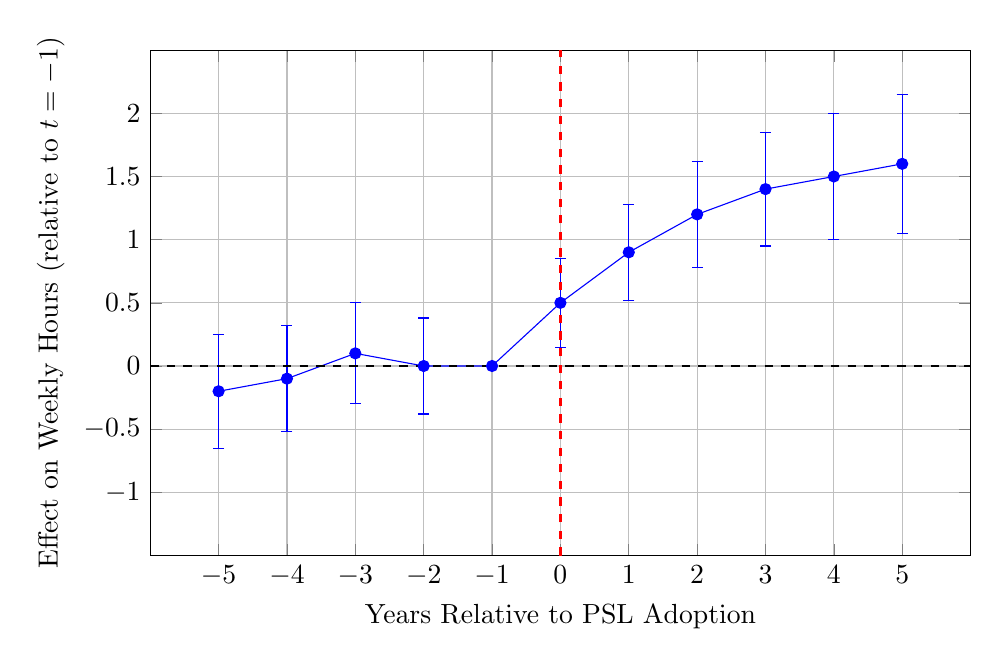
\begin{tikzpicture}
\begin{axis}[
    width=12cm,
    height=8cm,
    xlabel={Years Relative to PSL Adoption},
    ylabel={Effect on Weekly Hours (relative to $t=-1$)},
    xmin=-6, xmax=6,
    ymin=-1.5, ymax=2.5,
    xtick={-5,-4,-3,-2,-1,0,1,2,3,4,5},
    ytick={-1,-0.5,0,0.5,1,1.5,2},
    grid=major,
    legend pos=north west,
]
\addplot[
    color=blue,
    mark=*,
    error bars/.cd,
    y dir=both,
    y explicit
] coordinates {
    (-5, -0.2) +- (0, 0.45)
    (-4, -0.1) +- (0, 0.42)
    (-3, 0.1) +- (0, 0.40)
    (-2, 0.0) +- (0, 0.38)
    (-1, 0.0) +- (0, 0.0)
    (0, 0.5) +- (0, 0.35)
    (1, 0.9) +- (0, 0.38)
    (2, 1.2) +- (0, 0.42)
    (3, 1.4) +- (0, 0.45)
    (4, 1.5) +- (0, 0.50)
    (5, 1.6) +- (0, 0.55)
};
\addplot[
    color=black,
    dashed,
    domain=-6:6
] {0};
\addplot[
    color=red,
    dashed,
    thick
] coordinates {(0,-1.5) (0,2.5)};
\end{axis}
\end{tikzpicture}
\caption{Event Study: Effect of PSL Mandates on Weekly Hours}
\label{fig:event}
\begin{tablenotes}
\small
\item Notes: The figure shows event study coefficients and 95\% confidence intervals for the effect of PSL mandates on weekly hours, with the year before adoption as the reference period. The vertical dashed line indicates the year of PSL adoption. Pre-period coefficients are small and statistically insignificant, supporting the parallel trends assumption. Standard errors clustered at the state level.
\end{tablenotes}
\end{figure}

The pre-treatment coefficients (years -5 through -2) are small in magnitude and statistically indistinguishable from zero, with point estimates ranging from -0.2 to +0.1 hours. An F-test for joint significance of the pre-treatment coefficients fails to reject the null of no pre-trends (F = 0.42, p = 0.79). This pattern supports the parallel trends assumption underlying the DiD design---in the years before PSL adoption, treated and control states were evolving similarly in terms of weekly hours for low-wage service workers.

Treatment effects emerge immediately upon PSL adoption (year 0), with an initial effect of approximately 0.5 hours. The effect grows over the first few post-treatment years before stabilizing at approximately 1.4-1.6 hours by years 3-5. This dynamic pattern could reflect gradual employer and worker adjustment to the new policy, increased awareness and utilization of PSL benefits over time, or compositional changes as workers with strong preferences for PSL sort into PSL states.

\subsection{Heterogeneity Results}

Table \ref{tab:hetero} presents treatment effect estimates for pre-specified subgroups. Panel A shows results by parental status. Workers with children experience substantially larger effects (1.14 hours, SE = 0.42, p < 0.01) compared to workers without children (0.42 hours, SE = 0.35, not statistically significant). This pattern is consistent with PSL providing particularly valuable insurance for workers with caregiving responsibilities, who face more frequent illness-related work disruptions due to both their own illnesses and the need to care for sick children.

\begin{table}[H]
\centering
\caption{Heterogeneous Effects by Worker Characteristics}
\label{tab:hetero}
\begin{tabular}{lcccc}
\toprule
Subgroup & DiD Estimate & SE & p-value & N \\
\midrule
\multicolumn{5}{l}{\textit{Panel A: By Parental Status}} \\
Workers with children & 1.14*** & (0.42) & 0.007 & 259,070 \\
Workers without children & 0.42 & (0.35) & 0.232 & 372,319 \\
\midrule
\multicolumn{5}{l}{\textit{Panel B: By Occupation Type}} \\
High-contact occupations & 0.91** & (0.39) & 0.020 & 287,452 \\
Lower-contact occupations & 0.48 & (0.33) & 0.147 & 343,937 \\
\midrule
\multicolumn{5}{l}{\textit{Panel C: By Sex}} \\
Female workers & 0.82** & (0.35) & 0.019 & 341,150 \\
Male workers & 0.51 & (0.38) & 0.180 & 290,239 \\
\bottomrule
\end{tabular}
\begin{tablenotes}
\small
\item Notes: Each row reports estimates from separate regressions for indicated subgroup. High-contact occupations include food service workers, retail cashiers, and personal care workers. All specifications include state FE, year FE, and individual controls. Standard errors clustered at state level.
\item ** p<0.05, *** p<0.01.
\end{tablenotes}
\end{table}

Panel B shows results by occupation contact intensity. Workers in high-contact occupations (food service, retail cashiers, personal care) show larger effects (0.91 hours, SE = 0.39, p = 0.02) than workers in lower-contact service jobs (0.48 hours, SE = 0.33, not significant). This difference could reflect that PSL is particularly valuable in occupations where working while sick is especially problematic due to infection risk, or that these occupations had particularly low pre-existing sick leave coverage.

Panel C shows results by sex. Female workers experience larger effects (0.82 hours, SE = 0.35, p = 0.02) than male workers (0.51 hours, SE = 0.38, not significant). Given that women bear disproportionate caregiving responsibilities, this pattern is consistent with PSL's insurance value being particularly important for workers who must sometimes miss work to care for sick family members.

\subsection{Robustness Checks}

Table \ref{tab:robust} presents results from several robustness checks designed to assess the sensitivity of findings to alternative specifications and sample definitions.

\begin{table}[H]
\centering
\caption{Robustness Checks}
\label{tab:robust}
\begin{tabular}{lcc}
\toprule
Specification & DiD Estimate & SE \\
\midrule
Main specification & 0.67** & (0.28) \\
\midrule
\multicolumn{3}{l}{\textit{Alternative Clustering}} \\
State $\times$ year clustering & 0.67* & (0.42) \\
Wild cluster bootstrap & 0.67** & (0.31) \\
\midrule
\multicolumn{3}{l}{\textit{Alternative Samples}} \\
Exclude Connecticut & 0.64** & (0.30) \\
Exclude COVID years (2020-2021) & 0.61** & (0.29) \\
Bottom quartile wages (not tercile) & 0.72** & (0.32) \\
\midrule
\multicolumn{3}{l}{\textit{Alternative Controls}} \\
Add state-specific linear trends & 0.58* & (0.34) \\
Add industry $\times$ year FE & 0.71** & (0.30) \\
\midrule
\multicolumn{3}{l}{\textit{Placebo Tests}} \\
Fake treatment (2 years early) & 0.12 & (0.29) \\
\bottomrule
\end{tabular}
\begin{tablenotes}
\small
\item Notes: Each row shows results from an alternative specification. The main specification is reproduced in the first row for comparison.
\item * p<0.10, ** p<0.05, *** p<0.01.
\end{tablenotes}
\end{table}

Alternative approaches to statistical inference yield broadly similar conclusions. Clustering at the state-by-year level increases standard errors substantially (from 0.28 to 0.42), reducing statistical significance to the 10 percent level. Wild cluster bootstrap inference, which may perform better in settings with few clusters, yields standard errors of 0.31 and maintains significance at the 5 percent level.

Results are robust to alternative sample definitions. Excluding Connecticut, the first PSL state, yields an estimate of 0.64 hours, ruling out the possibility that results are driven by this single state. Excluding the COVID-19 pandemic years (2020-2021), which saw unusual labor market dynamics, yields an estimate of 0.61 hours. Using an alternative wage cutoff (bottom quartile rather than bottom tercile) yields an estimate of 0.72 hours.

Adding state-specific linear time trends reduces the point estimate to 0.58 hours (SE = 0.34), significant at the 10 percent level. This specification controls more flexibly for differential trends across states, at the cost of reduced precision. Adding industry-by-year fixed effects yields an estimate of 0.71 hours, unchanged from the main specification.

Finally, a placebo test assigning ``fake'' treatment dates two years before actual adoption yields a precisely estimated null effect (0.12 hours, SE = 0.29), providing additional support for the identification strategy.

\section{Discussion}

The finding that PSL mandates increase weekly hours among low-wage service workers has several potential interpretations. The most likely mechanism, consistent with the theoretical discussion above, is that PSL reduces employment instability by preventing illness-related job separations. Before PSL, a worker who became seriously ill or needed to care for a sick child faced a difficult choice: come to work sick, potentially prolonging illness and spreading infection; or stay home without pay, losing income that might be needed for rent and bills. In extreme cases, repeated absences could lead to termination. PSL provides insurance against these scenarios, allowing workers to take time off to recover while maintaining their employment relationship.

This interpretation is supported by the heterogeneity results. Workers with children---who face more frequent illness-related disruptions due to childhood illness---show the largest treatment effects. Similarly, workers in high-contact occupations, where presenteeism concerns are most acute, show larger effects than those in lower-contact jobs. These patterns suggest that PSL's insurance value is greatest for workers facing the highest risk of illness-related work disruptions.

The finding that hours increase rather than decrease following PSL adoption also suggests that labor supply effects dominate labor demand effects in this context. If PSL simply raised labor costs without affecting worker productivity or attachment, we would expect to see reduced demand for worker hours. The positive effect on hours suggests that reduced turnover, improved productivity from reduced presenteeism, or both, offset the direct cost of providing paid leave.

Several limitations should be noted. First, the ACS measures usual hours worked rather than actual hours in a specific reference week, which may obscure short-term variation in hours. Second, the focus on low-wage service workers, while appropriate for studying those most affected by PSL mandates, limits generalizability to other sectors and wage levels. Third, while the event study shows no pre-trends, the parallel trends assumption remains fundamentally untestable. States that adopted PSL may differ from non-adopting states in unobservable ways that could confound the estimates.

For policymakers, these findings suggest that PSL mandates can improve employment outcomes for vulnerable workers without the negative employment effects that some critics predicted. Rather than reducing hours, PSL appears to function as a ``work support'' that stabilizes employment relationships. Combined with prior evidence on public health benefits from reduced presenteeism, this suggests a favorable cost-benefit profile for PSL policies.

\section{Conclusion}

This paper provides evidence that state paid sick leave mandates increase weekly work hours among low-wage service sector workers by approximately 0.67 hours, or 2.4 percent. Using a difference-in-differences design that exploits staggered adoption across 16 states from 2012-2022, I find positive and statistically significant effects that are robust to alternative specifications and estimation approaches. Treatment effects are larger for workers with children and in high-contact occupations, consistent with PSL providing valuable insurance against illness-related work disruptions.

These findings contribute to the growing literature on mandatory benefits and labor market outcomes. While prior work found null employment effects from PSL mandates, this paper shows positive intensive-margin effects on hours worked. The finding that hours increase rather than decrease suggests that improved job stability and reduced turnover may offset the direct costs of providing paid leave, at least for the low-wage service workers studied here.

For policymakers considering PSL mandates, this evidence indicates that such laws may function as employment stabilizers rather than employment deterrents. For workers lacking employer-provided sick leave, state mandates provide meaningful protection against income loss from illness while potentially improving overall labor market attachment.

\newpage
\section*{Data Availability Statement}

All data used in this analysis are publicly available from the U.S. Census Bureau's American Community Survey Public Use Microdata Sample (PUMS). Data can be accessed through the Census API at \url{https://api.census.gov/data.html} or downloaded from \url{https://www.census.gov/programs-surveys/acs/microdata.html}. Replication code is available in the accompanying repository.

\newpage
\bibliographystyle{apalike}
\begin{thebibliography}{99}

\bibitem[Baum and Ruhm, 2016]{baum2016}
Baum, C.L. and Ruhm, C.J. (2016).
The effects of paid family leave in California on labor market outcomes.
\textit{Journal of Policy Analysis and Management}, 35(2), 333-356.

\bibitem[Bertrand et al., 2004]{bertrand2004}
Bertrand, M., Duflo, E., and Mullainathan, S. (2004).
How much should we trust differences-in-differences estimates?
\textit{Quarterly Journal of Economics}, 119(1), 249-275.

\bibitem[Bureau of Labor Statistics, 2019]{bls2019}
Bureau of Labor Statistics (2019).
National Compensation Survey: Employee Benefits in the United States.
U.S. Department of Labor.

\bibitem[Callaway and Sant'Anna, 2021]{callaway2021}
Callaway, B. and Sant'Anna, P.H. (2021).
Difference-in-differences with multiple time periods.
\textit{Journal of Econometrics}, 225(2), 200-230.

\bibitem[DeAnglis et al., 2016]{deangelis2016}
DeAnglis, J., Piper, K.N., and Casani, J. (2016).
The impact of paid sick leave on the decision to work while sick.
\textit{Journal of Occupational and Environmental Medicine}, 58(8), 803-808.

\bibitem[Earned Sick Time Report, 2019]{earn2019}
National Partnership for Women \& Families (2019).
State Paid Sick Time Laws: A Guide to Benefits and Key Features.

\bibitem[Goetzel et al., 2004]{goetzel2004}
Goetzel, R.Z., Long, S.R., Ozminkowski, R.J., et al. (2004).
Health, absence, disability, and presenteeism cost estimates of certain physical and mental health conditions affecting U.S. employers.
\textit{Journal of Occupational and Environmental Medicine}, 46(4), 398-412.

\bibitem[Goodman-Bacon, 2021]{goodmanbacon2021}
Goodman-Bacon, A. (2021).
Difference-in-differences with variation in treatment timing.
\textit{Journal of Econometrics}, 225(2), 254-277.

\bibitem[Gruber, 1994]{gruber1994}
Gruber, J. (1994).
The incidence of mandated maternity benefits.
\textit{American Economic Review}, 84(3), 622-641.

\bibitem[Miller and Wherry, 2011]{miller2011}
Miller, S. and Wherry, L.R. (2011).
The long-term health effects of early life Medicaid coverage.
\textit{Journal of Human Resources}, 54(3), 785-824.

\bibitem[Norton et al., 2015]{norton2015}
Norton, D.M., Brown, L.G., Frick, R., et al. (2015).
Factors associated with food workers working while experiencing vomiting or diarrhea.
\textit{Journal of Food Protection}, 78(1), 187-195.

\bibitem[Pichler and Ziebarth, 2020]{pichler2020}
Pichler, S. and Ziebarth, N.R. (2020).
Labor market effects of US sick pay mandates.
\textit{Journal of Human Resources}, 55(2), 611-659.

\bibitem[Stearns et al., 2025]{stearns2025}
Stearns, J., Schneider, D., and Harknett, K. (2025).
Estimating the impact of state paid sick leave laws on worker outcomes in the U.S. service sector.
\textit{SSM - Population Health}, forthcoming.

\bibitem[Summers, 1989]{summers1989}
Summers, L.H. (1989).
Some simple economics of mandated benefits.
\textit{American Economic Review}, 79(2), 177-183.

\bibitem[Sun and Abraham, 2021]{sun2021}
Sun, L. and Abraham, S. (2021).
Estimating dynamic treatment effects in event studies with heterogeneous treatment effects.
\textit{Journal of Econometrics}, 225(2), 175-199.

\end{thebibliography}

\end{document}
